%TODO 制作导航部分
\begin{withoutheadline}
\begin{frame}
\vspace*{-13mm}
\begin{figure}
	\hspace*{-4.2mm}
    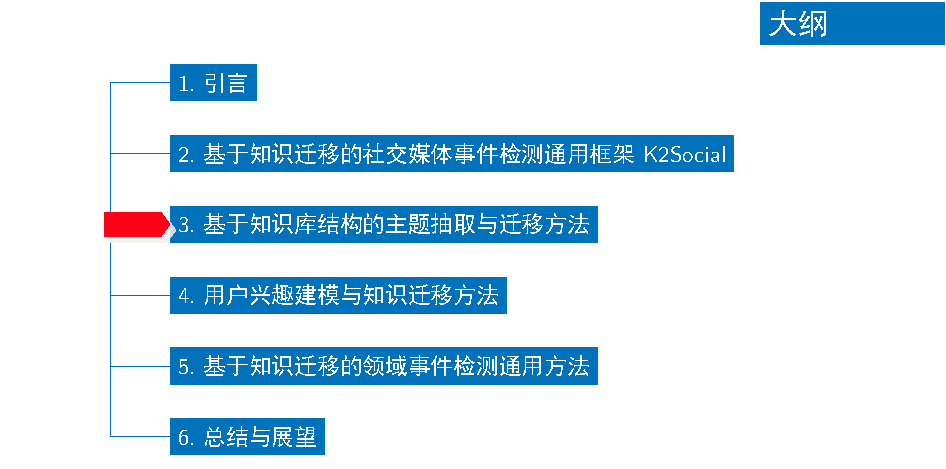
\includegraphics[width=1.0\paperwidth]{img/contents3_output.pdf}
\end{figure}

\end{frame}
\end{withoutheadline}

\section{基于知识库结构的主题抽取与迁移方法}
%\begin{frame}
%%\frametitle{\textsc{TransDetector}: Phase 1 (Extracting Category-Level Topics in KB) (3/3)}	
%%Taking the category \textit{Military} as an example, we extract \textit{Military}'s category-level topic \(\bm{h_{Military}}\).
%\begin{figure}[h]
%		\setlength{\abovecaptionskip}{0.cm}
%        \setlength{\belowcaptionskip}{0.cm}
%        \centering
%        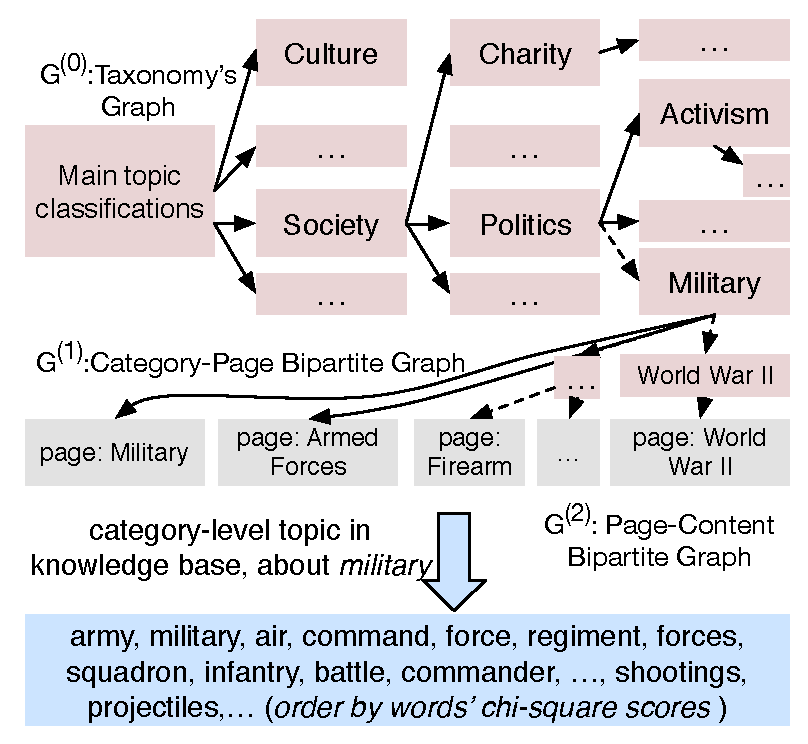
\includegraphics[width=0.7\columnwidth]{img/initializationExample.pdf}
%        %\caption{Extracting Category-Level Topics in Knowledge Base via its three fold hierarchical structure, taking \textit{Military} as an example.}
%        \label{fig:hood}
%\end{figure}
%\end{frame}

%\begin{frame}
%\frametitle{\textsc{TransDetector}: Phase 2 (Transferring Category-Level Info into Microblog Stream) (1/2)}	
%Transfer KB's Category-Level Topics \(\{\bm{h_c}\}_{c=1}^{K_{KB}}\) into microblogs stream: CTrans-LDA.
%\begin{figure}[h]
%		\setlength{\abovecaptionskip}{0.cm}
%        \setlength{\belowcaptionskip}{0.cm}
%        \centering
%        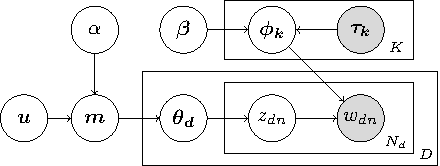
\includegraphics[width=0.6\columnwidth]{img/lda_tikz.pdf}
%        \caption{Diagram of CTrans-LDA.}
%        \label{fig:hood}
%\end{figure}
%
%In CTrans-LDA, \(\{\bm{h_c}\}_{c=1}^{K_{KB}}\) is used as prior information:
%\setlength{\abovedisplayskip}{0pt}
%\setlength{\belowdisplayskip}{0pt}
%\begin{scriptsize}
%\begin{equation}
%\label{eq:wikiPrior}
%\begin{aligned}
%\tau_{kv}=
%\left\{ \begin{aligned}
%\lambda \frac{h_{kv}}{\sum_{v\in S_{k}}h_{kv}} &,v\in S_{k}\ and  \ k \leq K_{\bm{KB}} \\
%0&,v \notin S_{k} \ or \ k > K_{\bm{KB}} \\
%\end{aligned}\right.
%\end{aligned}
%\end{equation}
%\end{scriptsize}
%\end{frame}

%\begin{frame}
%\frametitle{\textsc{TransDetector}: Phase 2 (Transferring Category-Level Info into Microblog Stream) (2/2)}	
%We use Gibbs Sampling for solving CTrans-LDA.
%\begin{itemize}
%	\item The initialization probability \(\hat{q}_{k|v}\) makes sure that the learned topics are aligned to the pre-defined category-level topic.
%\setlength{\abovedisplayskip}{0pt}
%\setlength{\belowdisplayskip}{0pt}
%\begin{scriptsize} 
%\begin{equation}
%\label{eq:initProbability}
%\begin{aligned}
%\hat{q}_{k|v}=
%\left\{ \begin{aligned}
%\frac{\tau_{kv}}{\sum_{k=1}^{K}\tau_{kv}} &,\sum_{k}\tau_{kv}>0 & (a)\\
%0&, \sum_{k}\tau_{kv}=0 \ and \ k \leq K_{\bm{KB}} & (b)\\
%1/(K-K_{\bm{KB}})&,\sum_{k}\tau_{kv}=0 \ and \ k > K_{\bm{KB}} & (c)
%\end{aligned}\right.
%\end{aligned}
%\end{equation}
%\end{scriptsize}
%\item Conditional probability in gibbs sampling:
%\(p(z_{dn}=k|.)\propto (n^{(d)}_{dk}+\alpha m_k)(n^{(w)}_{kv}+\tau_{kv}+\beta)/(n^{(w)}_{k,.}+\tau_{k,.}+V\beta)\).
%\end{itemize}
%\end{frame}

\begin{frame}
\frametitle{知识迁移提升事件检测性能的实例}	
%\noindent 在迁移学习之后的时间序列上,事件检测更易于进行
\begin{figure}[h]
		\setlength{\abovecaptionskip}{0.cm}
        \setlength{\belowcaptionskip}{0.cm}
        \centering
	\caption{词\textit{hood}的原始时间序列,与经过迁移学习之后的军事相关的\textit{hood}的时间序列对比图(在\textit{Edinburgh twitter corpus}数据集上计算)。相关事件可参考\url{https://en.wikipedia.org/wiki/Fort_Hood\#2011_attack_plot}.}
        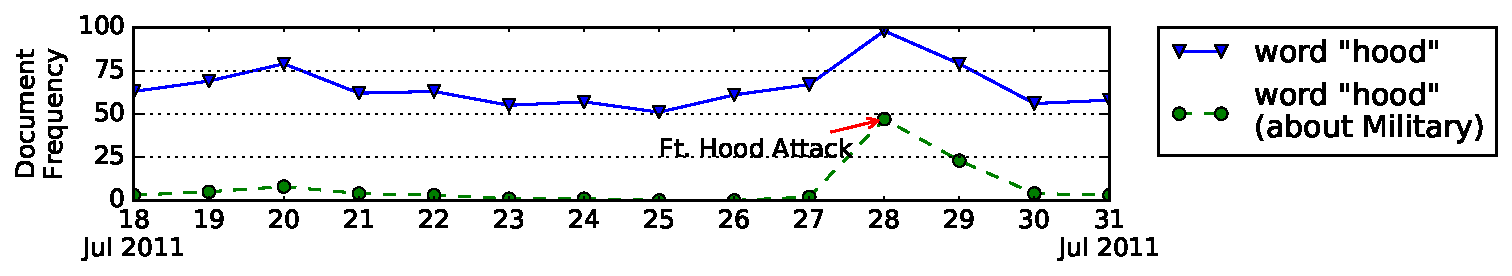
\includegraphics[width=1.0\columnwidth]{img/hood.pdf}
        \label{fig:hood}
\end{figure}

\begin{figure}[h]
	\setlength{\abovecaptionskip}{0.cm}
	\setlength{\belowcaptionskip}{0.cm}
	\centering
        \subfigure[常用词hood]{
                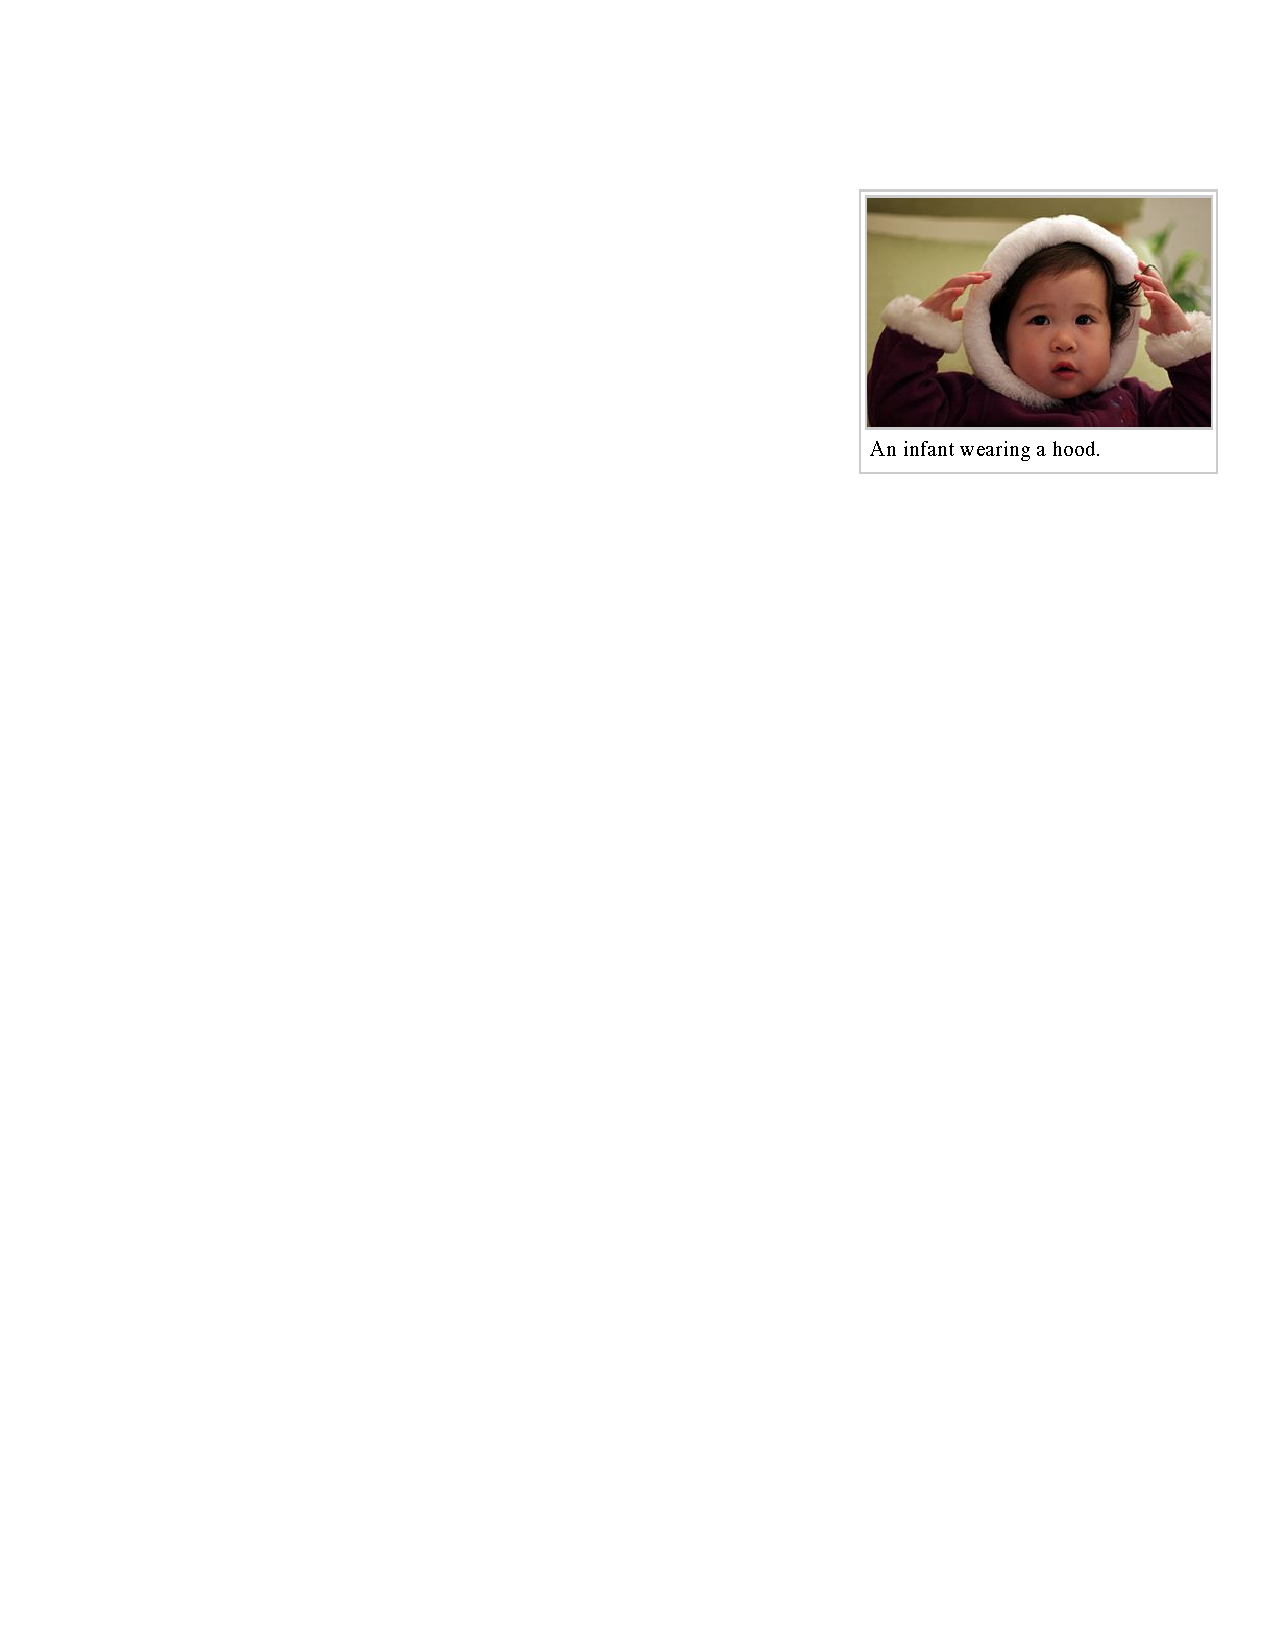
\includegraphics[height=2.12cm]{img/Hood(headgear)-Wikipedia.pdf}
        }
        \subfigure[和军事相关的词hood]{
                
\includegraphics[height=2.12cm]{img/Fort_Hood.pdf}
        }
\end{figure}
\end{frame}

\begin{frame}
\frametitle{我们的方法}
面向概念类的迁移学习方法\textsc{TransDetector},在K2Social框架下,分为三个阶段:
\vspace{-6mm}
\begin{columns}[t]
\column{0.26\textwidth}
\begin{enumerate}
	\item 主题抽取阶段 \\
	\item 迁移学习阶段 \\
	\item 事件检测阶段
\end{enumerate}

\column{0.74\textwidth}
\begin{figure}[h]
		\setlength{\abovecaptionskip}{-4mm}
        \setlength{\belowcaptionskip}{0.cm}
        \centering
		\caption{\textsc{TransDetector}三阶段处理流程}
        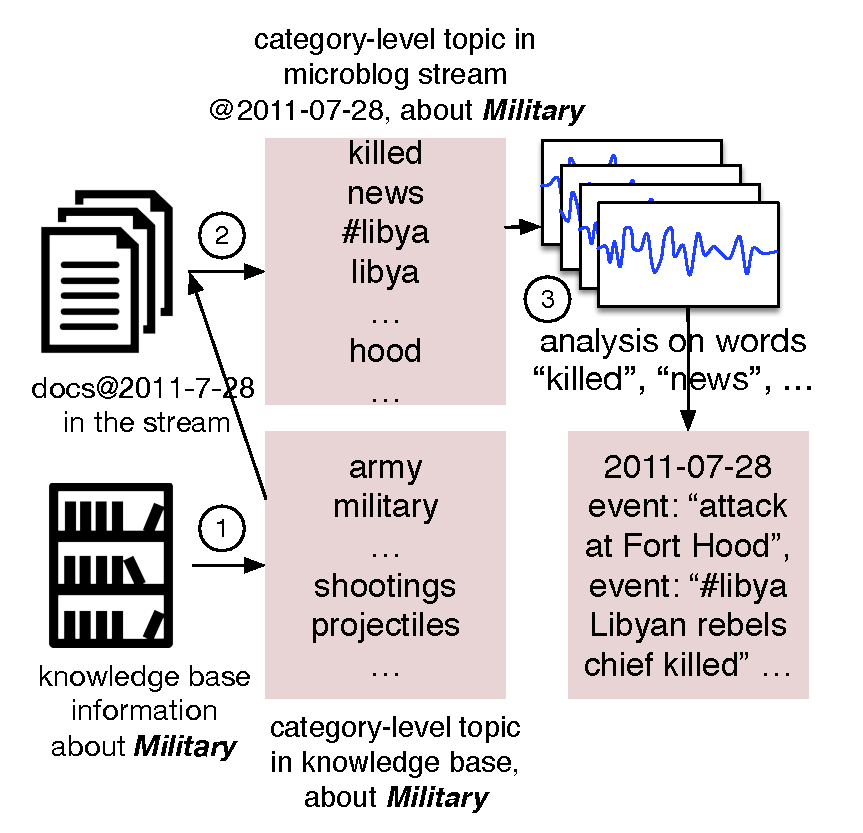
\includegraphics[width=0.7\columnwidth]{img/NSDetectorExample.pdf}
        \label{fig:hood}
\end{figure}
\end{columns}

\end{frame}


\begin{frame}
\frametitle{\textsc{TransDetector}:阶段3(在概念类别相关的词的时间序列上进行事件检测)(1/2)}	
\begin{figure}[h]
		\setlength{\abovecaptionskip}{0.cm}
        \setlength{\belowcaptionskip}{0.cm}
        \centering
        \caption{与\textit{Military}概念类相关的词的时间序列的气泡图示意,在\textit{Edinburgh Twitter Corpus}数据集上(2011年6月30日至2011年9月15日)进行实验,气泡图中的各个气泡圆圈的半径大小正比于词在对应时间窗口中的文档频率。}
        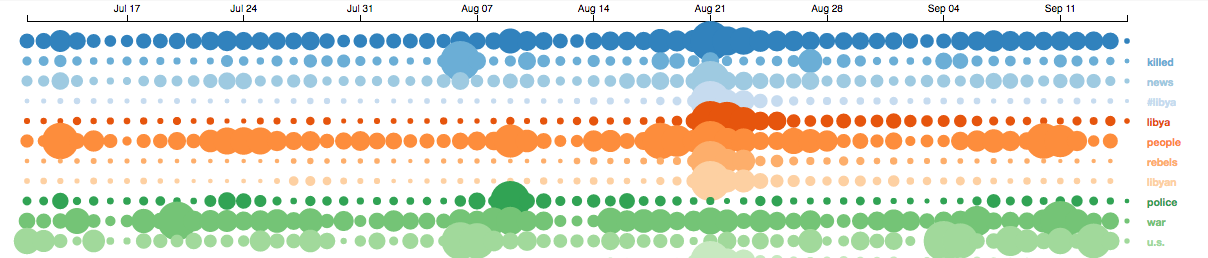
\includegraphics[width=.99\columnwidth]{img/screenShot.png}
        \label{fig:hood}
\end{figure}
\end{frame}

\begin{frame}
\frametitle{\textsc{TransDetector}:阶段3(在概念类别相关的词的时间序列上进行事件检测) (2/2)}
因自适应社交媒体语境动态演变,\textsc{TransDetector}能够更精确检测事件。
\begin{enumerate}
	\item 检测事件候选词
	\begin{itemize}
		\item 例如, \textit{Ft.}, \textit{Hood}, \textit{attack}.
	\end{itemize}
	\item 生成事件词组
	\begin{itemize}
		\item 例如, \textit{Ft. Hood attack}.
	\end{itemize}
	\item 召回事件相关的社交媒体文本
	\begin{itemize}
		\item 例如, \textit{Possible Ft. Hood Attack Thwarted \url{http://t.co/BSJ33hk}}.
	\end{itemize}
\end{enumerate}
\end{frame}


\begin{frame}
\frametitle{实验设置(1/3)}
\noindent 数据集
\begin{itemize}
	\item 知识库:英文维基百科\footnote{\tiny{\url{https://dumps.wikimedia.org/enwiki/latest/enwiki-latest-categorylinks.sql.gz}}}\ \footnote{\tiny{\url{https://dumps.wikimedia.org/enwiki/latest/enwiki-latest-pages-articles.xml.bz2}}},3,212,435篇维基页面,973,125个概念类别,\textsc{TransDetector}取$K_{\bm{KB}}=50$.
	\item 社交媒体数据流:Edinburgh twitter corpus\footnote{\tiny{\url{http://demeter.inf.ed.ac.uk/cross/docs/fsd_corpus.tar.gz}}},36,627,434条微博,时间跨度为2011年6月30日到2011年9月15日。
\end{itemize} 
对比方法
\begin{itemize}
	\item Twevent, BurstyBTM, LSH, EDCoW, TimeUserLDA
\end{itemize}
\end{frame}

\begin{frame}
\frametitle{实验设置(2/3)}
\noindent 事件评测基准
\begin{itemize}
	\item 基准1(Benchmark1): 随\textit{Edinburgh twitter corpus}数据集附带的手工标注的27个事件\footnote{\tiny{\url{http://demeter.inf.ed.ac.uk/cross/docs/Newswire_Events.tar.gz}}}.
\end{itemize}

\intextsep=5pt plus 3pt minus 1pt % 调整表格与正文的上间距
\begin{table}[]
\setlength{\abovecaptionskip}{-0.5cm}%set the distance between caption and table to 0 cm.
\setlength{\belowcaptionskip}{0.cm}
\centering
\caption{基准1中27个事件及对应的规模大小.}
\scalebox{0.42}{
\begin{tabular}{|l|l|r|}
\hline
Event                                        & Date       & Event Size \\ \hline
S\&P downgrade US credit rating                  & 05/08/2011 & 656      \\ \hline
Atlantis shuttle lands                           & 21/07/2011 & 595      \\ \hline
US increases debt ceiling                        & 25/07/2011 & 485      \\ \hline
Plane with Russian hocky team Lokomotiv crashes  & 07/09/2011 & 286      \\ \hline
Amy Winehouse dies                               & 23/07/2011 & 283      \\ \hline
Gunman opens fire in youth camp in Norway        & 23/07/2011 & 260      \\ \hline
Earthquake in Virginia                           & 24/08/2011 & 246      \\ \hline
First victim of London riots dies                & 09/08/2011 & 174      \\ \hline
Explosion in French nuclear plant in Marcoule    & 12/09/2011 & 135      \\ \hline
Google announces plans to bury Motorola Mobility & 15/08/2011 & 127      \\ \hline
NASA announces there might be water on Mars      & 04/08/2011 & 124      \\ \hline
Car bomb explodes in Oslo, Norway                & 22/07/2011 & 114      \\ \hline
... & ... & ... \\ \hline
\tikzmarkin<1>[hl]{bH1}Indian and Bangladesh sign a border pact         & 06/09/2011 & 25       \\ \hline
Flight 4896 crash                                & 13/07/2011 & 21       \\ \hline
First aritficial organ transplant                & 12/07/2011 & 18       \\ \hline
three men die in riots in england                & 10/08/2011 & 16       \\ \hline
rebels capture interational tripoli airport      & 21/08/2011 & 13       \tikzmarkend{bH1} \\ \hline
\end{tabular}
}
\end{table}

\begin{textblock*}{25mm}(93mm,75mm)
\noindent \tiny{11个事件的规模小于50(事件对应的微博少于50条)}
\end{textblock*}
\end{frame}

\begin{frame}
\frametitle{实验设置(3/3)}
\noindent 事件评测基准
\begin{itemize}
	%\item 基准1(Benchmark1): 随\textit{Edinburgh twitter corpus}数据集附带的手工标注的27个事件\footnote{\url{http://demeter.inf.ed.ac.uk/cross/docs/Newswire_Events.tar.gz}},{\color{red}但遗漏多个重要事件,如,“\textit{飓风艾琳登陆美国}”,“\textit{电影哈利波特与死亡圣器(下)上映}”等}。
	\item 基准2(Benchmark2): Twevent, BurstyBTM, LSH, EDCoW, TimeUserLDA, \textsc{TransDetector}提供的候选事件经人工和Current\_events\footnote{\tiny{\url{https://en.wikipedia.org/wiki/Portal:Current_events}}}对比,判断是否真实发生。总计{\color{red}395}个事件。
\end{itemize}
\vspace{-0.15cm}
\begin{figure}
\centering
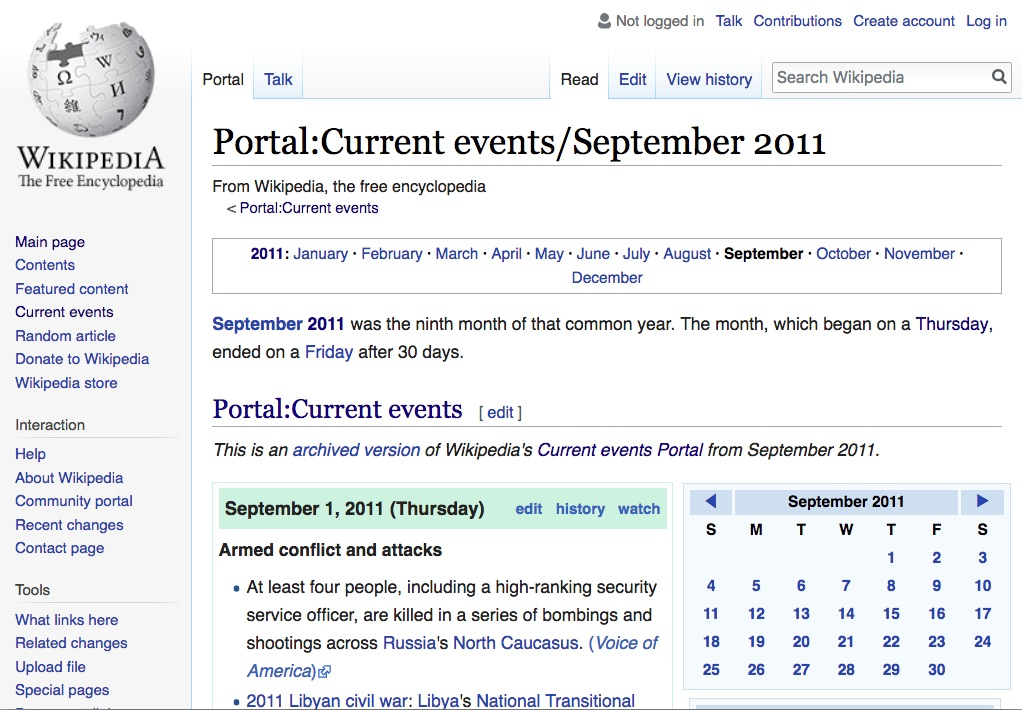
\includegraphics[height=4.7cm]{img/current_events.jpg}
\end{figure}
\end{frame}


\begin{frame}
\frametitle{实验结果:基于知识库结构的主题抽取质量}	
\begin{table}[h]
\setlength{\abovecaptionskip}{0.cm}%set the distance between caption and table to 0 cm.
\setlength{\belowcaptionskip}{0.cm}
\centering
\caption{以\textit{Aviation}概念类别为例,\textsc{TransDetector}抽取的相关主题与LightLDA(取主题个数为100)抽取的相关主题在主题连贯性(NPMI)指标上的对比。}
\scalebox{0.45}{
\begin{tabular}{|c|l|l|c !{\vrule width 1pt} c|l|l|c|}
\hline
\multicolumn{4}{|c!{\vrule width 1pt}}{Category-Level Topics extracted from Wikipedia by \textsc{TransDetector}} & \multicolumn{4}{c|}{Topics Learned from Wikipedia by LightLDA}    \\ \hline
GID& \#words*  & words  & NPMI & GID& \#words*& words & NPMI \\ \hline
- & 1-5 & aircraft air airport flight airline &-& - & 1-5 & engine aircraft car air power &-\\ \hline
0 & 1-5, 6-10 & \(\sim\), airlines aviation flying pilot squadron &  0.113 & 0 & 1-5, 6-10 & \(\sim\), design flight model production speed & 0.112\\ \hline
1 & 1-5, 11-15 & \(\sim\), flights pilots raf airways fighter & 0.155 & 1 & 1-5, 11-15 &\(\sim\), system vehicle cars engines mm & 0.062\\ \hline
2 & 1-5, 16-20 & \(\sim\), boeing runway force crashed flew   & 0.092 & 2 & 1-5, 16-20 & \(\sim\), fuel vehicles designed models type & 0.072\\ \hline
3 & 1-5, 21-25 &\(\sim\), airfield landing passengers plane aerial & 0.179 & 3 & 1-5, 21-25 & \(\sim\), version front produced rear electric & 0.035\\ \hline
4 & 1-5, 26-30 &\(\sim\), bomber radar wing bombers crash & 0.137 & 4 & 1-5, 26-30 & \(\sim\), space control motor standard development & 0.085\\ \hline
5 & 1-5, 31-35 &\(\sim\), airbus airports operations jet helicopter & 0.189 & 5 & 1-5, 31-35 & \(\sim\), film range light using available & -0.002\\ \hline
6 & 1-5, 36-40 &\(\sim\), squadrons base flown havilland crew & 0.088 & 6 & 1-5, 36-40 & \(\sim\), wing powered wheel weight launch & 0.087\\ \hline
7 & 1-5, 41-45 & \(\sim\), combat luftwaffe aerodrome carrier fokker & 0.159 & 7 & 1-5, 41-45 & \(\sim\), developed low test ford cylinder & 0.007\\ \hline
8 & 1-5, 46-50 &\(\sim\), planes fly engine takeoff fleet & 0.186 & 8 & 1-5, 46-50 & \(\sim\), equipment side pilot hp aviation & 0.091\\ \hline
9 & 1-5, 51-55 &\(\sim\), fuselage helicopters aviator naval aero & 0.157 & 9 & 1-5, 51-55 & \(\sim\), systems us sold body drive & -0.051\\ \hline
10 & 1-5, 56-60 &\(\sim\), glider command training balloon faa & 0.166 & 10 & 1-5, 56-60 & \(\sim\), gear introduced class safety seat & 0.069\\ \hline
\(\cdots\) & \(\cdots\) &\(\cdots\) &\(\cdots\) & \(\cdots\) & \(\cdots\) &\(\cdots\) &\(\cdots\)\\ \hline
18 & 1-5, 96-100 &\(\sim\), scheduled carriers military curtiss biplane &0.131 & 18 & 1-5, 96-100 & \(\sim\), transmission special replaced limited different & 0.059\\ \hline
19 & 1-5, 101-105 &\(\sim\), accident engines iaf albatross rcaf &0.068 & 19 & 1-5, 101-105 & \(\sim\), features machine nuclear even unit & 0.011\\ \hline
\end{tabular}
}
\label{tbl:NPMIDetails}
\end{table}

\end{frame}


\begin{frame}
\frametitle{实验结果:基于知识库结构的主题抽取质量}	
\begin{figure}[h]
	\setlength{\abovecaptionskip}{0.cm}
	\setlength{\belowcaptionskip}{0.cm}
        \centering
		\caption{对更多的\textsc{TransDetector}从维基百科抽取的概念类相关的主题的连贯性与LightLDA在维基百科上学习的主题连贯性进行对比。在前10个分组上,\textsc{TransDetector}显著更优。}
        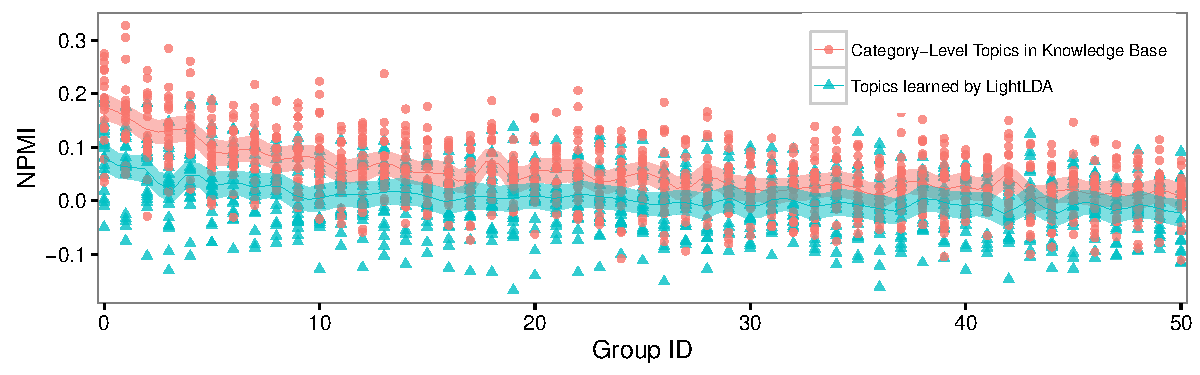
\includegraphics[width=1.0\columnwidth]{img/NPMI.pdf}
        \label{fig:NPMI}
\end{figure}
\end{frame}



%------------------------------
%page 2
\begin{frame}
\frametitle{实验结果:迁移学习效果}
\begin{table}
\setlength{\abovecaptionskip}{0.cm}%set the distance between caption and table to 0 cm.
\setlength{\belowcaptionskip}{0.cm}
\centering
\caption{CTrans-LDA迁移学习效果示例,展示从知识库中抽取的主题和经过迁移学习后微博中相关的主题。斜体标注的词为经过迁移学习后在\textit{社交媒体域}中学习到的和概念类别相关的新词。}
\scalebox{0.55}{
\begin{tabular}{|cc|cc|cc|cc|cc|cc|}
\hline
\multicolumn{2}{|c|}{\textit{Aviation}} & \multicolumn{2}{c|}{\textit{Health}} & \multicolumn{2}{c|}{\textit{Middle East}} & \multicolumn{2}{c|}{\textit{Military}} & \multicolumn{2}{c|}{\textit{Mobile Phones}}\\
\begin{tabular}[c]{@{}c@{}}Knowledge\\ Base\end{tabular} & \begin{tabular}[c]{@{}c@{}}Microblog\\ Stream\end{tabular} & \begin{tabular}[c]{@{}c@{}}Knowledge\\ Base\end{tabular} & \begin{tabular}[c]{@{}c@{}}Microblog\\ Stream\end{tabular} & \begin{tabular}[c]{@{}c@{}}Knowledge\\ Base\end{tabular} & \begin{tabular}[c]{@{}c@{}}Microblog\\ Stream\end{tabular} & \begin{tabular}[c]{@{}c@{}}Knowledge\\ Base\end{tabular} & \begin{tabular}[c]{@{}c@{}}Microblog\\ Stream\end{tabular} & \begin{tabular}[c]{@{}c@{}}Knowledge\\ Base\end{tabular} & \begin{tabular}[c]{@{}c@{}}Microblog\\ Stream\end{tabular} \\ 
\hline
aircraft & air & health & weight & al & \textbf{\textit{\#syria}} & army & killed & android & iphone\\ 
air & plane & patients & loss & israel & \textbf{\textit{\#bahrain}} & military & news & mobile & apple \\ 
airport & flight & medical & diet & iran & people & air & \textbf{\textit{\#libya}} & nokia & android \\ 
flight & time & disease & health & arab & israel & command & libya & ios & app \\
airline & airlines & treatment & cancer & israeli & police & force & rebels & phone & ipad \\
airlines & news & hospital & lose & egypt & \textbf{\textit{\#libya}} & regiment & people & samsung & samsung \\
aviation & boat & patient & fat & egyptian & \#egypt & forces & police & game & mobile\\
flying & airport & clinical & tips & ibn & news & squadron & war & app & blackberry \\
pilot & force & symptoms & treatment & jerusalem & \textbf{\textit{\#israel}} & infantry & libyan & iphone & tablet \\
squadron & fly & cancer & body & syria & world & battle & attack & htc & apps\\
\hline
\end{tabular}
}
\label{tbl:historyStates}
\end{table}
\end{frame}


\begin{frame}
\frametitle{实验结果:事件检测效果}	
\noindent \textsc{TransDetector}在保证召回率的同时,将准确率提升9\%

\begin{table}[h]
\setlength{\abovecaptionskip}{0.cm}%set the distance between caption and table to 0 cm.
\setlength{\belowcaptionskip}{0.cm}
\centering
\caption{在基于\textit{Edinburgh twitter corpus}数据集上构建的Benchmark1和Benchmark2,各个事件检测方法的性能对比}
\scriptsize
\scalebox{0.75}{
\begin{threeparttable}  
\begin{tabular}{|c|c|c|c|c|c|c|}
    \hline
    Method & \begin{tabular}[c]{@{}c@{}}Number of\\Events to \\ be Evaluated \end{tabular} & \begin{tabular}[c]{@{}c@{}}Recall@ \\ Benchmark1\end{tabular}& \begin{tabular}[c]{@{}c@{}}Precision@ \\ Benchmark2\end{tabular} & \begin{tabular}[c]{@{}c@{}}Recall@ \\ Benchmark2\end{tabular} & \begin{tabular}[c]{@{}c@{}}F@ \\ Benchmark2\end{tabular} & \begin{tabular}[c]{@{}c@{}}DERate\tnote{a}\ \ (Duplicate\\ Event Rate)@\\ Benchmark2\end{tabular} \\ \hline
    LSH & 500 & 0.704 & 0.788 & 0.651 & 0.713 & 0.348 \\ \hline
    TimeUserLDA & 100 & 0.370 & 0.790 & 0.177 & 0.289 & 0.114 \\ \hline
    Twevent & 375 &  0.741 & 0.808 & 0.658 & 0.725 & 0.142 \\ \hline
    EDCoW & 349 & 0.556 & 0.748 & 0.511 & 0.607 & 0.226 \\ \hline
    BurstyBTM & 200 & 0.667 & 0.825 & 0.384 & 0.497 & \textbf{0.079} \\ \hline
    \textsc{TransDetector} & 457 & \textbf{0.889} & \textbf{0.912} & \textbf{0.876} & \textbf{0.894} & 0.170 \\ \hline
    \end{tabular}

\begin{tablenotes}  
\item[a] DERate = (the number of duplicate events) / (the total number of detected realistic events)
\end{tablenotes}  
\end{threeparttable}  
}
\label{tbl:overall}
\end{table}
\end{frame}


\begin{frame}
\frametitle{实验结果:事件检测效果}
\noindent \textsc{TransDetector}在较小规模的事件上召回率明显高于已有方法。
\vfill
\begin{figure}[h]
	\setlength{\abovecaptionskip}{0.cm}
	\setlength{\belowcaptionskip}{0.cm}
        \centering
        \caption{在基于\textit{Edinburgh twitter corpus}数据集构建的Benchmark2上,召回率与事件规模之间的关系示意图}
        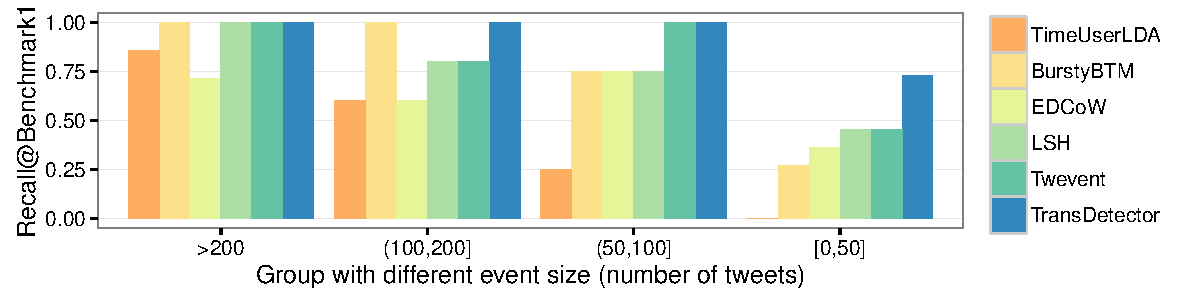
\includegraphics[width=1.0\columnwidth]{img/barchartOnBenchmark1.pdf}
        \label{fig:Benchmark1}
\end{figure}
\end{frame}

\begin{frame}
\frametitle{实验结果:事件检测效果}	
\noindent \textsc{TransDetector}在较小规模的事件上召回率明显高于已有方法。
\begin{table}
\setlength{\abovecaptionskip}{0.cm}%set the distance between caption and table to 0 cm.
\setlength{\belowcaptionskip}{0.cm}
\centering
\caption{2011-07-22至2011-07-28,\textit{Edinburgh Twitter Corpus}数据集中军事相关事件列表以及各事件检测方法的具体表现}
\vspace{-0.5cm}
\scalebox{0.6}{
\begin{threeparttable}  
\begin{tabular}{|c|l|l|c|c|c|c|c|c|c|}
\hline
\multirow{2}{*}{Date} & \multirow{2}{*}{Event key words} & \multirow{2}{*}{Representative event tweet} & \multirow{2}{*}{\begin{tabular}[c]{@{}l@{}}Number of \\ event tweet\end{tabular}} & \multicolumn{6}{c|}{Methods\tnote{a}} \\ \cline{5-10} 
 &  &  &  & L & TU & TW & E & B & TD \\ \hline
7/22/11 & \begin{tabular}[c]{@{}l@{}}Norway, Oslo,\\ attacks, bombing\end{tabular} & \begin{tabular}[c]{@{}l@{}}Terror Attacks Devastate Norway: A bomb\\ ripped through government offices in Oslo \\and a gunman... http://dlvr.it/cLbk8\end{tabular} & 557 & \checkmark & \checkmark & \checkmark & \checkmark & \checkmark & \checkmark \\ \hline
7/23/11 & Gunman, rink & \begin{tabular}[c]{@{}l@{}}Gunman Kills Self, 5 Others at Texas Roller\\ Rink http://dlvr.it/cLcTH\end{tabular} & 43 & - & - & \checkmark &  \checkmark & - & \checkmark \\ \hline
7/26/11 & \begin{tabular}[c]{@{}l@{}}Kandahar, mayor, \\ suicide, attack\end{tabular} & \begin{tabular}[c]{@{}l@{}}TELEGRAPH{]}: Kandahar mayor killed by\\ Afghan suicide bomber: The mayor of \\Kandahar, the biggest city in south \_\end{tabular} & 47 & \checkmark & - & \checkmark & \checkmark & - & \checkmark \\ \hline
7/28/11 & Ft., Hood, attack & \begin{tabular}[c]{@{}l@{}} Possible Ft. Hood Attack Thwarted\\ http://t.co/BSJ33hk\end{tabular} & 52 & - & - & - & - & - & \checkmark \\ \hline
7/28/11 & \begin{tabular}[c]{@{}l@{}}Libyan, rebel, \\ gunned\end{tabular} & \begin{tabular}[c]{@{}l@{}}Libyan rebel chief gunned down in Benghazi \\ http://sns.mx/prfvy1\end{tabular} & 44 & - & - & - & - & - & \checkmark \\ \hline
\end{tabular}

\begin{tablenotes}  
\item[a] L=LSH, TU=TimeUserLDA, TW=Twevent, E=EDCoW, B=BurstyBTM, TD=\textsc{TransDetector}.
\end{tablenotes}  
\end{threeparttable}  
}
\end{table}
\end{frame}

\begin{frame}
\frametitle{TransDetector方法小结}
\begin{columns}
\column{0.75\textwidth}

\begin{enumerate}
	\item 提出了一种以知识库结构为导向的概念类相关主题抽取方法;
	\item 提出了新的概率主题模型CTrans-LDA用于知识的迁移,并能自适应社交媒体的语境动态演变;
	\item 在知识迁移后的时间序列上进行事件检测,准确地检测社交媒体中蕴含的事件;
	\item Edinburgh Twitter Corpus数据集上准确率相较于目前已有的最佳方法提升了9\%
\end{enumerate}

\column{0.75\textwidth}

\end{columns}

\end{frame}
